\section{Introduction to Finite Difference and Finite Element Approximations}
\label{sec:intr-finite-ele-diff}

The finite difference and finite element methods allow the \emph{discretisation} of a continuous differential equation to allow for solution by computational methods. The finite element method allows for more complex geometries than the finite difference method, at the cost of increased complexity and setup time.

A simple problem is used to illustrate these methods: solving the Poisson
equation in one spatial dimension. Find\footnote{A function $g\in C^{k}(0,1)$ if $g$ and it's first $k$ derivatives are continuous on $(0,1)$.} $y(x)\in C^{2}(0,1)$ such that
\begin{equation}
  -y''=f\qquad\text{on }(0,1)
  \label{eq:poisson1}
\end{equation}
\begin{equation*}
  y(0)=y_{a},\quad y(1)=y_{b},\quad f=f(x)\in C(0,1).
\end{equation*}

\subsection{Finite Difference Approximation}
\label{sec:finite-diff-appr}

We start with the equation~\eqref{eq:poisson1} and subdivide this interval into
$N$ sub intervals each of length $h = \frac{1}{N}$ as shown in Figure
\ref{fig:The-subdivision}. The points $x_{i}$ are the points where we will
approximate $y(x)$ (i.e. we will compute a discrete solution $y(x_{i})$ for
$i=0, \, \ldots \, ,N$).

\begin{figure}[!ht]
  \center
  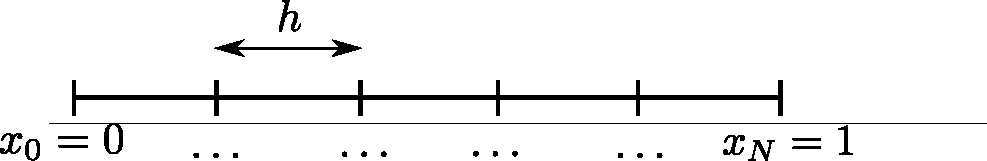
\includegraphics[width=1\textwidth]{./images/finite_diff_discretisation}
  \caption{Subdivision of the unit interval for finite difference approximation.}
  \label{fig:The-subdivision}
\end{figure}

The Taylor series for a function $y(x)$ at a point $x$ near $a$
is defined as
\begin{equation*}
  y(x)=y(a)+y'(a)(x-a)+\dfrac{y''(a)}{2!}(x-a)^{2}
  + \dfrac{y'''(a)}{3!}(x-a)^{3}+\dfrac{y^{(4)}(a)}{4!}(x-a)^{4}\ldots.
\end{equation*}

Using $a=x_{i}$ and $x=x_{i+1}$ we get
\begin{equation}
  y(x_{i+1})=y(x_{i})+hy'(x_{i})+\dfrac{h^{2}}{2}y''(x_{i})+\dfrac{h^{3}}{3!}y'''(a)+O(h^{4}),
  \label{eq:taylor1}
\end{equation}
where $O(h^{4})$ is the residual. Similarly for $x=x_{i-1}$
\begin{equation}
  y(x_{i-1})=y(x_{i})-hy'(x_{i})+\dfrac{h^{2}}{2}y''(x_{i})-\dfrac{h^{3}}{3!}y'''(a)+O(h^{4}).
  \label{eq:taylor2}
\end{equation}

Adding equations~\eqref{eq:taylor1} and \eqref{eq:taylor2} gives
\begin{equation*}
  y(x_{i+1})+y(x_{i-1})=2y(x_{i})+h^{2}y''(x_{i})+O(h^{4}).
\end{equation*}
We then rearrange to get an expression for $y''(x_{i})$ in terms of $y$:
\begin{equation*}
  y''(x_{i})=\dfrac{1}{h^{2}}\Big[y(x_{i+1})+y(x_{i-1})-2y(x_{i})\Big]+O(h^{4}).
  % Milan says error is O(h^{4}) but I can't see why it's not O(h^{2})...
\end{equation*}

We now drop the $O(h^{4})$ term leaving an approximation for $y''(x_{i})$
\begin{equation}
  y''(x_{i})=\dfrac{1}{h^{2}}\Big[y(x_{i+1})+y(x_{i-1})-2y(x_{i})\Big],
  \label{eq:y''approx}
\end{equation}

with an error of order $h^{4}$ (so the error rapidly decreases with small
sub intervals). Similar manipulation of the Taylor series can be used to obtain
other derivatives of $y$ for use when solving differential equations other than
the Poisson equation. For example $y'$ can be found by subtracting equation
\eqref{eq:taylor2} from equation~\eqref{eq:taylor1}.

Substituting the approximations for $y''(x_{i})$ from equation~\eqref{eq:y''approx}
into \eqref{eq:poisson1} at each $x_{i}$ gives a set of $n$ linear
equations for the unknowns $y(x_i) = y_i \, (i=1 , \, \ldots \, , n)$

\begin{equation*}
  \dfrac{1}{h^{2}}\Big[y(x_{i+1})-2y(x_{i})+y(x_{i-1})\Big]=-f(x_{i}).
\end{equation*}

We introduce a shorthand notation often used in this area: $y_{i}=y_{h}(x_{i})$
and $f_{i}=f(x_{i})$. Multiplying by $-1$ and changing to the new
notation gives
\begin{equation}
  \dfrac{1}{h^{2}}\Big[-y_{i+1}+2y_{i}-y_{i-1}\Big]=f_{i}.
  \label{eq:23}
\end{equation}

So far we have not included the boundary conditions in \eqref{eq:23}. We know
from the problem specification that $y(x_{0})=y_{a}$ and $y(x_{n+1})=y_{b}$.  A
simple way to enforce these conditions is to include them as two additional
trivial equations in our linear system. For example the linear system
approximating the Poisson equation at three points (since $y(x_{0})$ and
$y(x_{4})$ are known) is then:

\begin{equation*}
  \dfrac{1}{h^{2}}\left[
    \begin{array}{ccccc}
      h^{2} & 0 & 0 & 0 & 0\\
      -1 & 2 & -1 & 0 & 0\\
      0 & -1 & 2 & -1 & 0\\
      0 & 0 & -1 & 2 & -1\\
      0 & 0 & 0 & 0 & h^{2}
    \end{array}
  \right]\left[
    \begin{array}{c}
      y_{0}\\ y_{1}\\ y_{2}\\ y_{3}\\ y_{4}
    \end{array}
  \right]  =  \left[
    \begin{array}{c}
      y_{a}\\ f_{1}\\ f_{2}\\ f_{3}\\ y_{b}
    \end{array}
  \right],
\end{equation*}

which simplifies to

\begin{equation}
  \dfrac{1}{h^{2}}\left[
    \begin{array}{ccc}
      2 & -1 & 0\\
      -1 & 2 & -1\\
      0 & -1 & 2
    \end{array}
  \right]\left[
    \begin{array}{c}
      y_{1}\\ y_{2}\\ y_{3}
    \end{array}
  \right]=\left[
    \begin{array}{c}
      f_{1}+y_{a}/h^{2}\\ f_{2}\\ f_{3}+y_{b}/h^{2}
    \end{array}
  \right].
  \label{eq:simple-linear-eq-finite-diff-1}
\end{equation}

This can be easily solved computationally by using standard linear algebra solvers.


\subsubsection{Example}

\begin{figure}[!ht]
  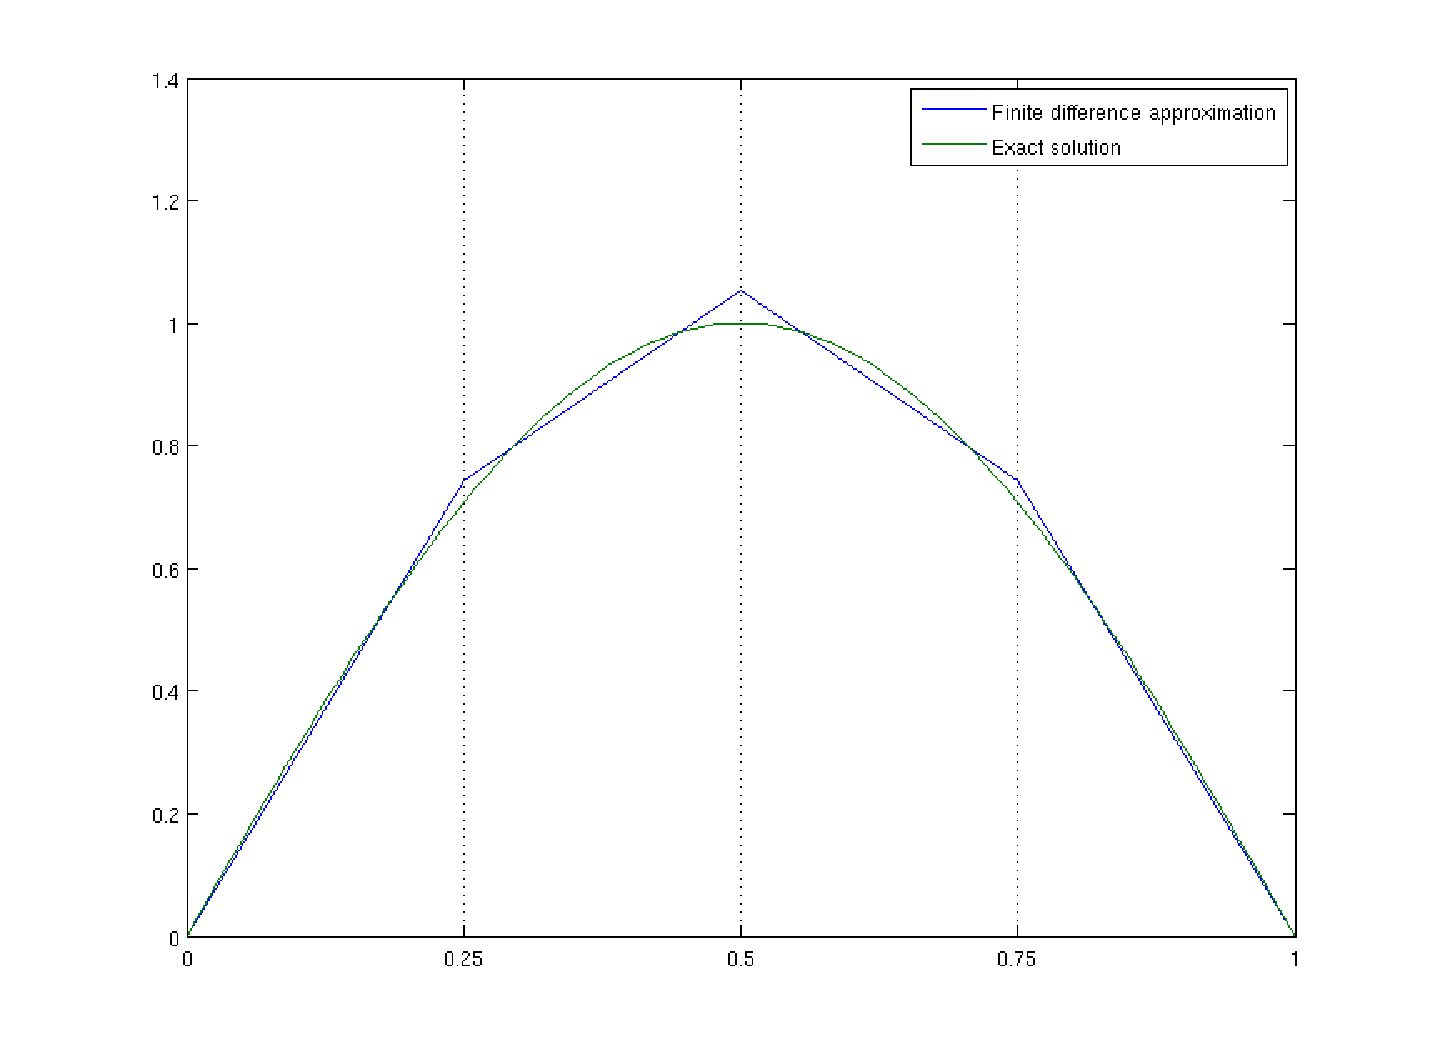
\includegraphics[width=1\textwidth]{./images/finitediffexample}
  \caption{A finite difference approximation for $y''(x)=-\pi^{2}\sin(\pi x)$,
    $y(0)=0$ and $y(1)=0$ for $x\in[0,1]$. The exact solution is $y(x)=\sin(\pi x)$.}
  \label{fig:A-finite-difference-example}
\end{figure}

We will use an $f(x)$ which corresponds to an exact solution. Let
$y(x)=\sin(\pi x)$, then $f(x)=\pi^{2}\sin(\pi x)$, $y(0)=0$ and
$y(1)=0$. Let $N=5$, then the linear system to be solved is:

\begin{equation*}
  \dfrac{1}{(0.25)^{2}}\left[
    \begin{array}{ccc}
      2 & -1 & 0\\
      -1 & 2 & -1\\
      0 & -1 & 2
    \end{array}
  \right]\left[
    \begin{array}{c}
      y_{1}\\ y_{2}\\ y_{3}
    \end{array}
  \right] = \left[
    \begin{array}{c}
      \dfrac{\pi^{2}}{\sqrt{2}}+0\\
      \pi^{2}\\
      \dfrac{\pi^{2}}{\sqrt{2}}+0
    \end{array}
  \right].
\end{equation*}

Solving for $\mathbf{y} = [ y_1, y_2, y_3]$ gives
\begin{equation*}
  \left[
    \begin{array}{c}
      y_{1}\\ y_{2}\\ y_{3}
    \end{array}
  \right]=\left[
    \begin{array}{c}
      0.74\\ 1.05\\ 0.74
    \end{array}
  \right],
\end{equation*}
which is plotted in Figure~\ref{fig:A-finite-difference-example}.


\subsection{Finite Elements}
\label{sec:finite-elements-one-d}

\subsubsection{Definitions}
\label{sec:fem-definitions}

The function space $L^{2}$ is the set of all functions $f(x)$ such
that $\intop_{-\infty}^{\infty}|f(x)|^{2}dx$ is finite.

The span of a set of functions is the set of all possible linear combinations of
the functions. If a set of functions $\{\phi_{i}\}$ is such that
$V=\text{span}(\phi_{i})$ then we say that $\{\phi_{i}\}$ spans $V$ and
$\{\phi_{i}\}$ is a basis for the function space $V$. If $V$ has a basis consisting of a finite number of functions then we say that $V$ is finite dimensional, otherwise $V$ is infinite dimensional.

In finite element models we are interested in approximating an infinite
dimensional space (the space of solutions) by a finite dimensional
space (the space of approximations).

The $n$-th Sobelov space is the space of all functions such that they and their $n$-th derivatives (in all dimensions) are in $L^2$. For example
\begin{equation}
  \label{eq:H1}
  \sob^1(\magd) = \{ y \st y, \pd{y}{x_i} \in L^2(\magd) \; \forall x_i \}
\end{equation}

\subsubsection{The Weak Formulation \& A Discretisation}
\label{Derivation-of-weighted-residuals}

The method of weighted residuals is a way to convert a differential equation
into an integral form that can be modelled computationally. As such it is the
first step in a variety of modelling methods including the finite element method
and the spectral method.

For simplicity we start, as before, with the one-dimensional Poisson equation
\eqref{eq:poisson1}, with homogeneous Dirichlet boundary conditions
(i.e. $y_{a}=y_{b}=0$).

% \footnote{The functions must be Lipschitz continous (a stronger form
%   of continuity than standard). Lipschitz continuity is defined as the
%   following: for $X,Y$ metric spaces with metrics $d_{x}(x_{1},x_{2})$,
%   $d_{y}(y_{b},y_{2})$ respectively then a function $f:X\rightarrow Y$ is
%   Lipschitz continuous if and only if $\exists K\geq0$ s.t. $\forall
%   x_{1},x_{2}\in X$ $d_{y}(f(x_{1}),f(x_{2}))\leq K\, d_{x}(x_{1},x_{2})$.}

The formulation used in \eqref{eq:poisson1} is too restrictive for our purposes:
it disallows some useful approximating functions, and in higher dimensional
cases restricts the domain shapes that can be modelled
\cite{HowardElmanDavidSilvester2006}. However for well behaved functions the
following \emph{weak formulation} is equivalent: find $y\in V_{s}$ such that
\begin{equation}
  -\int_{0}^{1}y''v\, dx=\int_{0}^{1}fv\, dx \qquad \forall v\in V_{T}.
  \label{eq:26}
\end{equation}

Here $V_{T}$ is some appropriate space of \emph{test functions}. The test
functions must satisfy $V_{T}\subseteq \sob^0(0,1)$, in order to ensure that the integrals in \eqref{eq:26} are well defined. Thus
\begin{equation}
  \label{eq:28}
  V_{T}=\{v:[0,1]\rightarrow\mathbb{R}\, \st \, v \in \sob^0(0,1)\}.
\end{equation}

The space $V_{s}$ is the solution space
\begin{equation*}
  V_{s}=\{y:[0,1]\rightarrow\mathbb{R}\, \st \, y \in \sob^2(0,1),\,
  y(0) = y_{a},\, y(1) = y_{b}\},
\end{equation*}
 i.e. the space of functions that are sufficiently smooth for the integrals to be finite and that satisfy the boundary conditions.

To see that the weak form is equivalent consider the case when the error or \emph{residual} $f(x) -y(x)''$ is non-zero for some $x \in [0,1]$. Since equation~\eqref{eq:26} must hold for all functions $v$ we can come up with a function which is non-zero at $x$ and hence the equality in \eqref{eq:26} fails. We call this the method of weighted residuals because we use a weighted integral of the residual to approximate the true equation.\cite{Zeinkiewicz1967}%pg 210,214

The smoothness restrictions on our weak form approximation can be further reduced using integration by parts
\begin{equation*}
  \int_{0}^{1}q\, dp=\Big[pq\Big]_{0}^{1}-\int_{0}^{1}p\, dq,
\end{equation*}
applied to the left hand side of equation~\eqref{eq:26}. Let $p=y'$ and $q=v$, then
\begin{equation}
  -\int_{0}^{1}y''v\, dx=-\Big[y'v\Big]_{0}^{1}+\int_{0}^{1}y'v'\, dx.
  \label{eq:29}
\end{equation}

We now introduce a second constraint to the test functions: $v=0$
at the boundaries (i.e. $v_a=v_b=0$), so the bracketed term in \eqref{eq:29} is
zero and we are left with
\begin{equation*}
  -\int_{0}^{1}y''v\, dx=\int_{0}^{1}y'v'\, dx.
\end{equation*}

Hence our problem can be reduced to the following: find $y\in V_{S}'=\{y \st \, y \in \sob^1(0,1),\, y(0) = y_a, y(1) = y_b \}$
such that
\begin{equation}
  \int_{0}^{1}y'v'\, dx=\int_{0}^{1}fv\, dx\qquad\forall v\in V'_{T}=\{v \st \, v \in \sob^1(0,1),\, v_a=v_b=0\}.\label{eq:symmetric-weak-poisson}
\end{equation}

Note that this rearrangement has removed the second derivative in $y$, hence we only require $y \in \sob^1(0,1)$ instead of $y \in \sob^2(0,1)$. This allows a wider range of shape
functions to be used but comes at the expense of requiring more smoothness in
the test functions. Also note that if $y_a = y_b = 0$ then $V_{S}'=V_{T}'$, our
test and solution spaces are the same.

Equation~\eqref{eq:symmetric-weak-poisson} is still inapplicable as a
computational method since the test (and solution) space is infinite dimensional
(i.e. the problem is still continuous). So for the next step we approximate
$V_{T}'$ by a finite dimensional function space $V_{T}^{h}\subset V_{T}'$ such
that
\begin{equation}
  V_{T}^{h}=\text{span} \{ \tbf_{\ndi} \}_{n=1}^{N}
  =  \{v_h \st v_h = \sum_{n=0}^{N}\alpha_{\ndi} \tbf_{\ndi},\, \alpha_{\ndi} \in \real,\, v_a = v_b =0 \},
  \label{eq:30}
\end{equation}
for some finite set of basis functions $\tbf_{\ndi}$. Similarly for $V_S$
\begin{equation}
  \label{eq:34}
    V_{S}^{h}=\text{span} \{ \sbf_{l} \}_{l=1}^{N_l}
    =  \{y_h \st y_h = \sum_{l=0}^{N_l}c_{l} \sbf_{l},\,
    c_{l} \in \real,\, y(0) = y_a,\, y(1) = y_b \}.
\end{equation}

We call $\sbf_l$ the \emph{shape functions}. The choice of $\tbf_{\ndi}$
and $\sbf_l$ lead to different modelling methods, the choice corresponding
to the finite element method will be discussed in section \ref{sub:Actual-Finite-Elements}. For now we convert the problem into a general discrete form.

We currently have the \emph{discrete weak formulation} of \eqref{eq:poisson1}: find $y_{h}\in V_{S}^{h}$ such that
\begin{equation}
  \int_{0}^{1}y'_{h}v_{h}'\, dx=\int_{0}^{1}fv_{h}\, dx\qquad\forall v_{h}\in V_{T}^{h}.
  \label{eq:discrete-weak-prob}
\end{equation}

Replacing $v_{h}$ from \eqref{eq:discrete-weak-prob} by $\tbf_{\ndi}$
gives
\begin{equation}
  \int_{0}^{1} y'_{h} \tbf_{\ndi}' \, dx = \int_{0}^{1}f\tbf_{\ndi}\, dx\qquad n=0,\ldots,N,
  \label{eq:discrete_weak_test_fns_replaced}
\end{equation}

Since $y_{h}\in V_{S}^{h}$ we can also replace $y_{h}$ by a linear combination
of the spanning functions, i.e.
\begin{equation}
  y_{h}=\sum_{l=0}^{N_l}c_{l}\sbf_{l},
  \label{eq:y-spans}
\end{equation}
where $c_l \in \real$ are the (unknown) coefficients.

Substituting \eqref{eq:y-spans} into equation~\eqref{eq:discrete_weak_test_fns_replaced} gives
\begin{equation}
  \sum_{l=0}^{N_l}c_{l}\int_{0}^{1}\sbf_{l}'\tbf'_{\ndi}\, dx=\int_{0}^{1}f\tbf_{\ndi}\, dx
  \qquad n=0,\ldots,N.
  \label{eq:31}
\end{equation}

The functions $f$, $\tbf$ and $\sbf$ are known and so the integrals in \eqref{eq:31} are just numbers (which must be explicitly calculated at some point). Hence we introduce a matrix $A$ and a vector $\mathbf{b}$ containing these numbers:
\begin{equation}
  \int_{0}^{1}\sbf_{l}'\tbf'_{\ndi}\, dx=A_{l\ndi},\qquad\int_{0}^{1}f\tbf_{\ndi}\, dx=b_{j},\label{eq:Aij_bj}
\end{equation}
and the problem is reduced to a system of linear equations
\begin{equation}
  A\mathbf{c} = \mathbf{b}.
  \label{eq:final_galerkin}
\end{equation}
This can be solved to find the vector of unknown coefficients $\mathbf{c}$ which can be substituted into \eqref{eq:y-spans} to give an approximation for $y$.


\subsubsection{Finite Elements in One Dimension}
\label{sub:Actual-Finite-Elements}

To create a useable implementation of the methodology derived in Section~\ref{Derivation-of-weighted-residuals} we must first define a set of basis functions $\tbf_\ndi$ for the space $V_{T}^{h}$ and a set of $\sbf_l$ for the space $V_S^h$. For simplicity we choose the two types of basis functions to be the same: $\sbf_l = \tbf_l$. This choice defines the Galerkin method (and often results in symmetric matrix $A$).\cite{Zeinkiewicz1967} %pg215


The overall aim is to approximate an arbitrary function at a finite set of \emph{nodes}, $x_\ndi$, by a linear combination of a finite set of simple functions, $\tbf_\ndi$. There are a variety of useful choices for $\tbf_\ndi$ but we will focus on a carefully constructed set of polynomials -- the Lagrange interpolation basis functions, defined as
\begin{equation*}
  L_\ndi(x)=\prod_{k\neq i}\Bigg(\dfrac{x-x_{k}}{x_\ndi-x_{k}}\Bigg).
\end{equation*}

This definition results in the following useful properties of $L_{\ndi}(x)$
\begin{equation}
  \label{eq:35}
  L_{\ndi}(x_{\ndi}) =
  \begin{cases}
    1 & k = \ndi, \\
    0 & k \neq \ndi,
  \end{cases}
\end{equation}
since at each $x_{\ndi}$ with $k \neq \ndi$ one of the numerators is zero and at
$x_{\ndi}$ all of the numerators are equal to the corresponding denominator.

Polynomials are chosen because they are easy to manipulate computationally, for example differentiation and integration are simple. Also an arbitrary level of accuracy can be achieved when approximating the a smooth function by piecewise polynomials, provided that the polynomials are only non-zero on a sufficiently small area (i.e. after sufficient mesh refinement).

We now consider the simple case where we approximate the function at two points
$x_{0}$ and $x_{1}$ (linear interpolation). Then the Lagrange basis
functions are simply
\begin{equation}
  L_{0}=\dfrac{x-x_{1}}{x_{0}-x_{1}},\qquad
  L_{1}=\dfrac{x-x_{0}}{x_{1}-x_{0}}.
  \label{eq:simple_lagrange}
\end{equation}
The interpolation of a function on the interval $[x_{0},x_{1}]$ is then given by
\begin{equation*}
  y_{h}(x)=y(x_{0})L_{0}(x)+y(x_{1})L_{1}(x).
\end{equation*}

It is advantageous to work with such simple functions even for very complex
models because evaluation of integrals and interpolation is quick and easy. We
can achieve this by splitting the domain into a set of $N$ \emph{elements}
$e_{0},e_{1},\ldots,e_{N-1}$, which can be of varying size (in contrast to the
basic finite difference method where the nodes had to be equally spaced). We
then create a \emph{local} numbering scheme for the nodes and functions in each
element and a \emph{global} numbering scheme to keep track of the same nodes and
functions over the entire domain.

In one dimension the boundary of each element consists of two points, one at
each end. In the local scheme it is natural to label these points by the element
number $e$ and a local node number, i.e. $x_{0}^{(e)}$ and $x_{1}^{(e)}$. In the
global scheme each node is labelled by a unique node number, i.e. $x_{\ndi}$ for
$\ndi=0,\ldots,N$. The concept is best illustrated by a diagram, see Figure
\ref{fig:local-global-numbering}.

\begin{figure}[ht]
  \center
  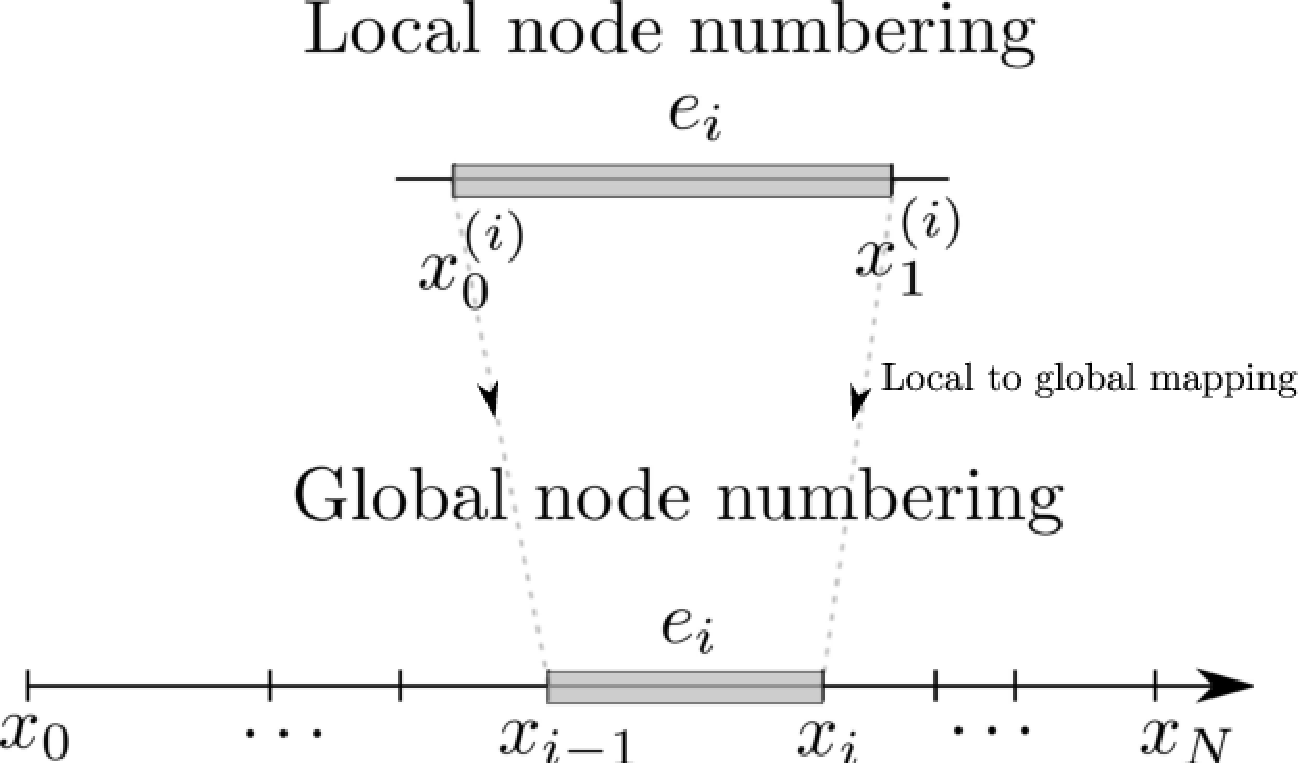
\includegraphics[width=0.8\textwidth]{./images/local_global_numbering}
  \caption{The local and global numbering schemes for nodes in a one-dimensional
    finite element model.}
  \label{fig:local-global-numbering}
\end{figure}

The process of assigning a global node number to each local node is known as the
local to global mapping. Good book keeping of the mapping is essential,
especially in higher dimensions when this it becomes much more complex.

We define the local basis functions in element $e$ as
\begin{equation}
  L_{0}^{(e)}(x)=\dfrac{x-x_{1}^{(e)}}{x_{0}^{(e)}-x_{1}^{(e)}},\qquad
  L_{1}^{(e)}(x)=\dfrac{x-x_{0}^{(e)}}{x_{1}^{(e)}-x_{0}^{(e)}}
  \qquad\text{for }x\in e=[x_{0}^{(e)},x_{1}^{(e)}].
  \label{eq:32}
\end{equation}
Except for the test functions when $\ndi$ is a boundary node. In this case we define $L_\ndi^{(e)} = 0$.
The $\ndi$th global basis function is then defined as:
\begin{equation}
  \label{eq:33}
  L_\ndi(x) =
  \begin{cases}
    L_\ndi^{(e)}(x) & \text{if node $\ndi$ is in element $e$,} \\
    0 & \text{otherwise.}
  \end{cases}
\end{equation}

\begin{figure}[!ht]
  \center
  % ??ds numbering: change e_i to element e, e_{i+1} to e+1, x_i to x_\ndi, x^(i) to x^(e) L_i to L_\ndi
  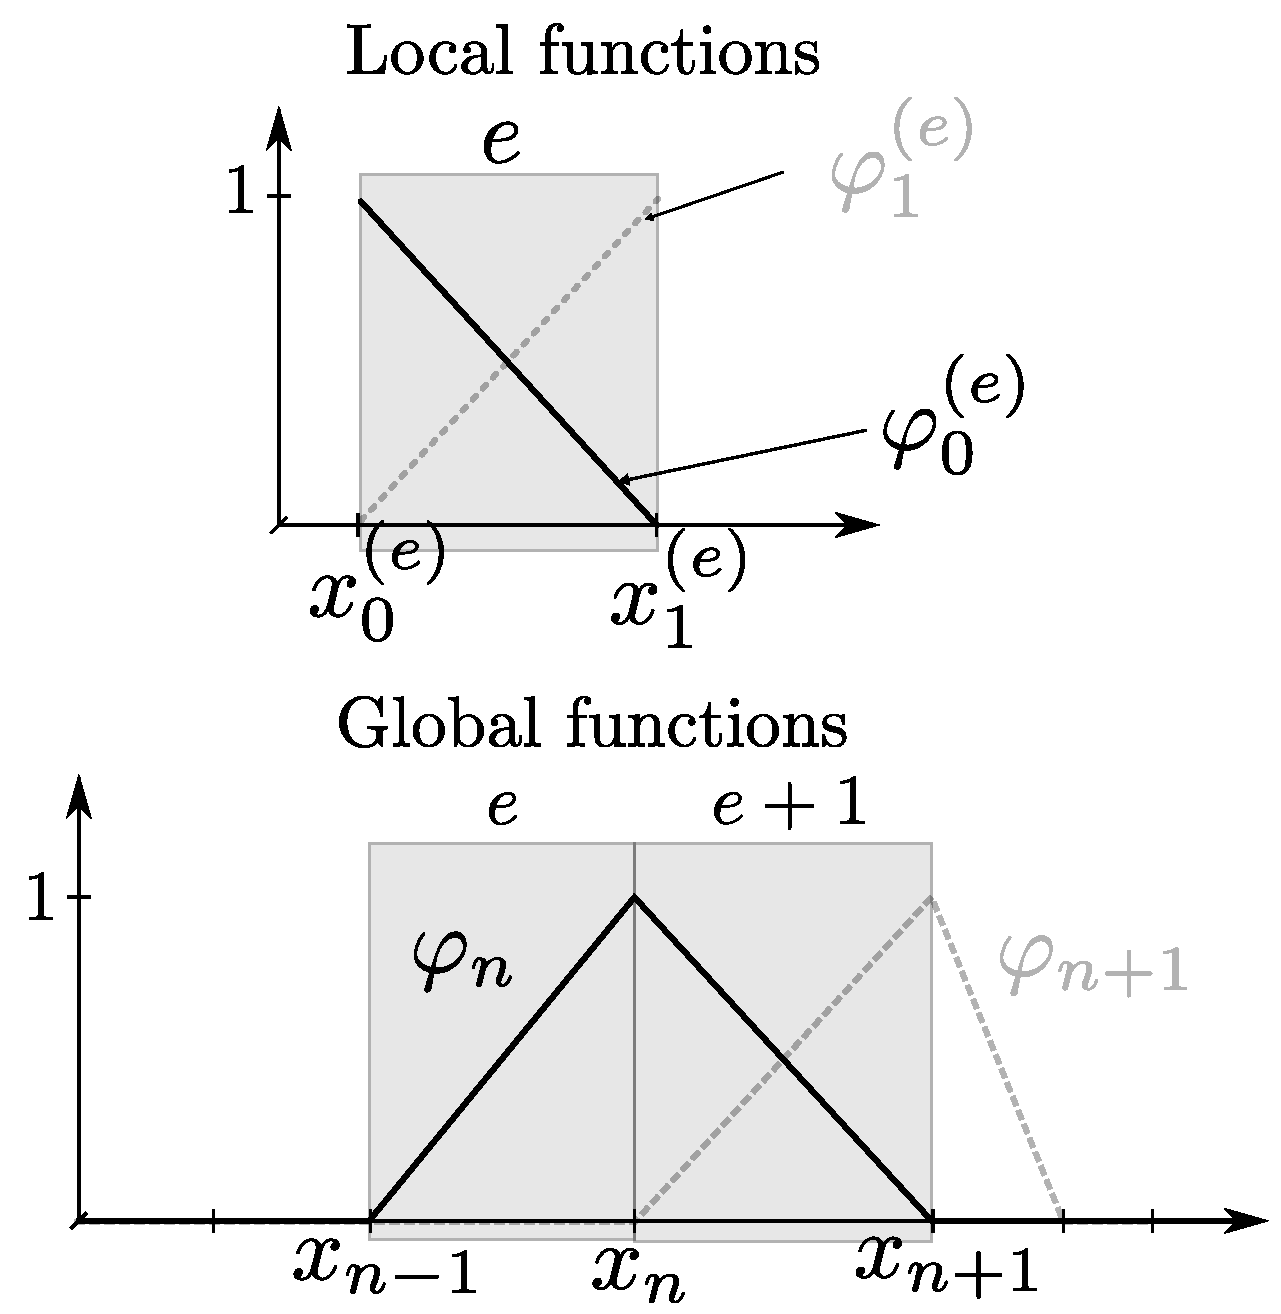
\includegraphics[width=0.8\textwidth]{./images/local_global_functions}
  \caption{The linear Lagrange basis functions and numbering schemes for a one-dimensional
    finite element model.\label{fig:local_global_functions}}
\end{figure}

The global basis functions for are clearly integrable (i.e. in $L^2[0,1]$) since
they are just a combination of local basis functions and they satisfy the boundary conditions by definition. So the global basis functions are members of $V_T^h$ and $V_S^h$.

To calculate the matrix $A$ and the vector $\mathbf{b}$ from equation
\eqref{eq:Aij_bj} needed for \eqref{eq:final_galerkin} we first calculate the
local contributions from each element: $A^{(e)}$ and $\mathbf{b}^{(e)}$. Then the
local-to-global mapping tells us which local nodes map to a given global node
and so the global $A$ and $\mathbf{b}$ can be assembled by summing the
appropriate local contributions.

For our one-dimensional Poisson case the calculation of $A^{(e)}$ is quite
simple, substituting the two local basis functions \eqref{eq:32} into
\eqref{eq:Aij_bj} and using $h=x_{1}^{(e)}-x_{0}^{(e)}$ we are left with
\begin{equation*}
  A^{(e)} = \dfrac{1}{h}
  \left[
    \begin{array}{cc}
      1 & -1 \\ -1 & 1
    \end{array}
  \right],
\end{equation*}
where $h$ is the element size, $h = x_{1}^{(e)}-x_{0}^{(e)}$ (note that $h$ can
vary between elements). Similarly for $\mathbf{b}^{{e}}$ we obtain
\begin{equation*}
  \mathbf{b}^{(e)}=\dfrac{1}{h}\left[
    \begin{array}{c}
      -\int_{x_{0}^{(e)}}^{x_{1}^{(e)}}(x-x_{1}^{(e)})\, f(x)\, dx\\
      \int_{x_{0}^{(e)}}^{x_{1}^{(e)}}(x-x_{0}^{(e)})\, f(x)\, dx
    \end{array}\right],
\end{equation*}
which we compute numerically since the entries depend on $f(x)$ which is not yet
decided.


\subsection{Extensions of the Finite Element Method}

\subsubsection{Non-Dirichlet Boundary Conditions}
\label{sub:Non-Dirichlet-Boundary-Conditions}

There are two main types of boundary condition. Dirichlet conditions specify the
\emph{value} at the boundary (as used so far). Neumann conditions specify the
\emph{derivative} at the boundary. These two types can also be mixed together
either as conditions on different parts of the boundary or as a linear
combination of the two (a Robin condition).

Neumann boundary conditions can be added to the finite element method described
above by relaxing the conditions on the shape and test functions at the
boundary. Then the first term in equation~\eqref{eq:29} naturally gives an
additional equation for the Neumann condition on each boundary node.

Combinations of Neumann and Dirichlet conditions on different parts of the boundary can be treated the same way, by restricting the shape and test functions only on the Dirichlet parts.


\subsubsection{Other Equations}
\label{sec:fem-other-equations}

Finite element models are used to solve a wide range of equations including for example applications in fluid/solid mechanics, electrostatics and magnetostatics. There can be various subtleties in the application to different equations but the main difference in the method described so far is the derivation of the weak form. However the same steps of multiplying by a test function and transferring derivatives to the test functions are still used.


\subsubsection{Higher Order Shape/Test Functions}
\label{sec:fem-high-order-shap}

The shape and test functions can also be chosen to be of quadratic, cubic or higher order. This increases the number of nodes required per element (to ensure uniqueness) and increases the difficulty of calculating the integrals. However in some cases the use of higher order polynomials can give a better approximation.


\subsubsection{Higher Dimensions}
\label{sec:fem-higher-dimensions}

The same basic method as given in Sections~\ref{Derivation-of-weighted-residuals} and \ref{sub:Actual-Finite-Elements} can be applied to two and three dimensional problems. Different polynomials for the shape/test functions must be chosen but the basic orthogonality property from equation~\eqref{eq:35} is kept. A larger variety of element shapes are possible -- typically triangular or quadrilateral elements are used in two dimensions and their higher dimension equivalents (tetrahedrons and ``bricks'') are used in three dimensions.


%%% Local Variables:
%%% mode: latex
%%% TeX-master: "./main"
%%% End:
